\section{Segunda iteración}

En esta segunda iteración pretendemos mejorar algunos de los aspectos que nos hemos encontrando en la primera, o aspectos que simplemente hemos dejado para después. Comenzaremos con una alternativa al balanceo de
datos, y luego probaremos otros tipos tanto de aprendizaje como de modelos.

\subsection{Balanceo de datos}\ \label{sec:i2-balance}

La toma de nuevos datos es costosa y como tenemos relativamente pocos datos para la cantidad de columnas, el balanceo de datos es esencial. En la primera iteración, intentamos sortear este problema utilizando métricas
 

La toma de nuevos datos reales es costosa, y como teníamos relativamente pocos datos para entrenar el balanceo es esencial. Podemos hacer unos entrenamientos y comparar los resultados para ver si es necesario 
balancear, los resultados los podemos ver en la \textit{tabla\ \ref{tab:balanced_comparison}}. Fijándonos en las columnas a partir de \textit{f1score}, ya que estas son las métricas que ignoran el balanceo de 
los datos, podemos ver que, son mejores los modelos entrenados sobre el \gls{dataset} balanceado.

\begin{table}[!ht]
    \centering
    \resizebox{\textwidth}{!}{\begin{tabular}{|c|ccccc|ccccc|} \hline
    & \multicolumn{5}{|c|}{Balanced dataset} & \multicolumn{5}{c|}{Unbalanced dataset} \\ \hline
    Model Name & Train score & Test score & f1score & f0.5score & Balanced accuracy & Train score & Test score & f1score & f0.5score & Balanced accuracy \\ \hline
    XGBoost model & 92.051 & 87.669 & 87.055 & 89.736 & 87.669 & 82 & 82 & 0 & 0 & 50 \\
    Stochastic Gradient Descent & 79.584 & 78.862 & 76.506 & 81.988 & 78.862 & 46.37 & 47.778 & 34.54 & 25.985 & 59.003 \\
    Random Forest model & 94.399 & 87.398 & 86.58 & 90.09 & 87.398 & 99.926 & 85.333 & 35.294 & 54.545 & 60.705 \\
    Quadratic Discriminant Analysis & 87.94 & 87.669 & 86.191 & 92.871 & 87.669 & 81.778 & 79.333 & 34.043 & 37.383 & 59.937 \\
    Multi-Layer Perceptron & 89.205 & 85.908 & 85.014 & 88.376 & 85.908 & 86.889 & 81.111 & 17.476 & 26.627 & 53.794 \\
    Linear Discriminant Analysis & 82.746 & 80.759 & 78.743 & 84.026 & 80.759 & 82.815 & 80.667 & 2.247 & 4.425 & 49.669 \\
    LightGBM model & 92.141 & 87.127 & 86.409 & 89.402 & 87.127 & 57.778 & 52 & 39.665 & 29.857 & 65.914 \\
    K-Neighbors model & 100 & 83.333 & 81.048 & 88.314 & 83.333 & 100 & 85.111 & 46.4 & 56.42 & 65.869 \\
    Hist Gradient Boosting model & 82.294 & 81.436 & 79.764 & 84.322 & 81.436 & 73.556 & 62 & 33.463 & 27.389 & 58.522 \\
    Extra Trees model & 86.224 & 84.688 & 82.695 & 89.701 & 84.688 & 95.481 & 83.111 & 52.5 & 52.897 & 70.912 \\
    Decision Tree model & 80.352 & 79.268 & 76.279 & 83.503 & 79.268 & 82 & 82 & 0 & 0 & 50 \\ \hline
    \end{tabular}}
    \caption{Tabla comparativa de los resultados de entrenar los modelos con los datos balanceados y sin balancear, después de preprocesar los datos. Fuente propia.}\ \label{tab:balanced_comparison}
\end{table}

Para balancear el \gls{dataset}, hacemos dos procedimientos: \textit{undersampling} y \textit{oversampling}. Como su nombre indica, \textit{undersampling} es una técnica para reducir las muestras de la clase mayoritaria, en nuestro caso los granos sin contaminar. Para ello, utilizamos la librería \href{https://imbalanced-learn.org/stable/}{imblearn} que fue diseñada específicamente para la clasificación de clases desbalanceadas. En ella, podemos encontrar diferentes algoritmos para reducir las muestras de la clase que queramos de los cuales nos hemos quedado con los \href{https://imbalanced-learn.org/stable/references/generated/imblearn.under_sampling.EditedNearestNeighbours.html}{EditedNearestNeighbours}. Este algoritmo en resumen elimina las muestras que no se parezcan demasiado a sus vecinos\ \cite{Wil72}. Para hacer \textit{oversampling} utilizamos la librería \href{https://sdv.dev/}{sdv}, más específicamente el \href{https://docs.sdv.dev/sdv/single-table-data/modeling/synthesizers/gaussiancopulasynthesizer}{GaussianCopulaSynthesizer}, el cual utiliza métodos estadísticos clásicos para generar datos sintéticos parecidos a los reales. Una vez generados los datos sintéticos, podemos comprobar su calidad generando un reporte de calidad de la con la misma librería \textit{sdv}, utilizando la función \href{https://docs.sdv.dev/sdv/single-table-data/evaluation#evaluate_quality}{evaluate\_quality} la cual compara los datos generados con los reales y nos da los resultados de la \textit{figura\ \ref{fig:quality_report}}.

\begin{figure}[!ht]
    \centering
    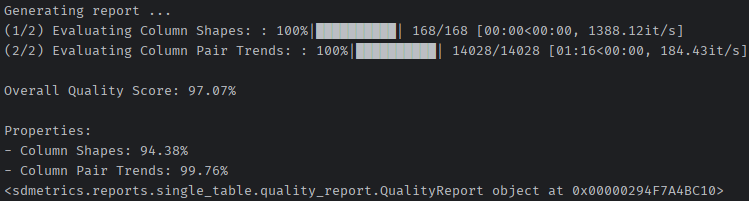
\includegraphics[width=0.8\linewidth]{media/images/quality_report.png}
    \caption{Reporte de calidad de los datos generados sintéticamente, fuente propia.}\ \label{fig:quality_report}
\end{figure}

Una vez aplicados los dos algoritmos obtenemos un \gls{dataset} balanceado como el de la \textit{figura\ \ref{fig:balance}}.

\begin{figure}[!ht]
    \centering
    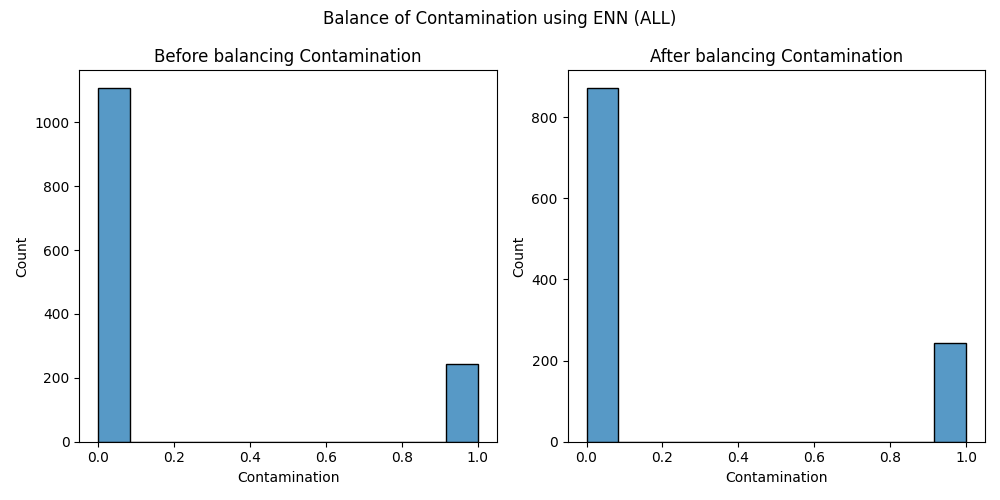
\includegraphics[width=0.6\linewidth]{media/images/balance.png}
    \caption{Comparación del balanceo de la clase objetivo del \gls{dataset} antes y después de balancear, fuente propia, código\ \ref{code:plots_balancing}}\ \label{fig:balance}
\end{figure}